\documentclass[12pt,a4paper]{article}
\usepackage[utf8]{inputenc}
\usepackage[T1]{fontenc}
\usepackage{amsmath}
\usepackage{amsfonts}
\usepackage{amssymb}
\usepackage{graphicx}
\usepackage[margin=2cm]{geometry}
\usepackage{subcaption}
\usepackage[french]{babel}
\usepackage{multicol}
\usepackage{listingsutf8}
\usepackage{listings}
\usepackage{float}
\usepackage{notoccite}
\usepackage{url}

%

\usepackage{color}

\lstset{inputencoding=latin1}
\definecolor{mygreen}{rgb}{0,0.6,0}
\definecolor{mygray}{rgb}{0.5,0.5,0.5}
\definecolor{mymauve}{rgb}{0.58,0,0.82}
\lstset{ %
	backgroundcolor=\color{white},   % choose the background color; you must add \usepackage{color} or \usepackage{xcolor}; should come as last argument
	basicstyle=\footnotesize,        % the size of the fonts that are used for the code
	breakatwhitespace=false,         % sets if automatic breaks should only happen at whitespace
	breaklines=true,                 % sets automatic line breaking
	captionpos=b,                    % sets the caption-position to bottom
	commentstyle=\color{mygreen},    % comment style
	deletekeywords={...},            % if you want to delete keywords from the given language
	escapeinside={\%*}{*)},          % if you want to add LaTeX within your code
	extendedchars=true,              % lets you use non-ASCII characters; for 8-bits encodings only, does not work with UTF-8
	frame=single,	                   % adds a frame around the code
	keepspaces=true,                 % keeps spaces in text, useful for keeping indentation of code (possibly needs columns=flexible)
	keywordstyle=\color{blue},       % keyword style
	language=Octave,                 % the language of the code
	morekeywords={*,...},            % if you want to add more keywords to the set
	numbers=left,                    % where to put the line-numbers; possible values are (none, left, right)
	numbersep=5pt,                   % how far the line-numbers are from the code
	numberstyle=\tiny\color{mygray}, % the style that is used for the line-numbers
	rulecolor=\color{black},         % if not set, the frame-color may be changed on line-breaks within not-black text (e.g. comments (green here))
	showspaces=false,                % show spaces everywhere adding particular underscores; it overrides 'showstringspaces'
	showstringspaces=false,          % underline spaces within strings only
	showtabs=false,                  % show tabs within strings adding particular underscores
	stepnumber=2,                    % the step between two line-numbers. If it's 1, each line will be numbered
	stringstyle=\color{mymauve},     % string literal style
	tabsize=2,	                   % sets default tabsize to 2 spaces
	title=\lstname,% show the filename of files included with \lstinputlisting; also try caption instead of title
	rangeprefix= ,% curly left brace plus space
	rangesuffix=% space plus curly right brace               
}

%title
\usepackage{titling}
\newcommand{\mytitle}{Projet : Multicores embarqué pour Big Data et
	Machine Learning}
\author{\textbf{DOU Yuhan\\ FORCIOLI Quentin \\ GHAOUI Mohamed Anis\\  TERRACHER Audrey}}

%header
\usepackage{fancyhdr}
\usepackage{lastpage}
\fancyhf{}
\lhead{\leftmark}
\rfoot{Page \thepage\ sur \pageref{LastPage}}


%hypersetup
\usepackage{hyperref}
\hypersetup{
	colorlinks=true,
	linkcolor=black,
	filecolor=magenta,      
	urlcolor=black,
	pdftitle={\mytitle},
	pdfauthor=GHAOUI Mohamed Anis,
	pdfpagemode=Maximize,
	citecolor=black,
}

%listings
\usepackage{minted}

%figures
\usepackage{caption}
\usepackage{subcaption}



\begin{document}
\begin{titlepage}
\begin{center}
\vspace*{1cm}

\textbf{Master E3A}

\vspace{0.5cm}


Cours A2 : Systèmes Electroniques Embarqués

\vspace{1.5cm}
\mytitle

\vspace{1.5cm}
\theauthor

\vspace{1.5cm}
Encadré par :
\textbf{HAMMAMI Omar} et \textbf{LE PROVOST Hervé}
\vfill

Master 2 : Système Embarqué et Traitement de l'Information\\
\vspace{0.8cm}
Année : 2019-2020
\vspace{0.8cm}
\begin{center}
	
\includegraphics[width=0.4\textwidth]{logo}
	
\includegraphics[width=0.4\textwidth]{logo2}
\end{center}


\end{center}
\end{titlepage}

\newpage
\tableofcontents
\newpage
\listoffigures
\newpage
\pagestyle{fancy}
\section{Introduction}
Durant le siècle dernier, les algorithmes sont passés d'une sombre idée à la base de toutes choses faites. Ces algorithmes traitent les données à leur entrée dans des temps parfois constant, consistant et parfois moins déterminés quand ils sont exécutés de manière totalement séquentielle. Avec la récente explosion du Big Data, ces algorithmes doivent traiter de plus en plus des données de plus en plus volumineuse et multi-dimensionnelles. Il est évident qu'une solution parallèle doit être déployée afin de répondre à une telle demande. 

On propose alors de concevoir des architectures pouvant effectuer un calcul parallèle utilisant le principe simple qu'une implémentation matérielle est toujours plus rapide, à fréquence égale, qu'une implémentation logicielle. Le problème est que la conception de ces implémentation par des outils de synthèse demande beaucoup de ressources humaine et de réflexions afin de produire un résultat correct et performant. On pense alors à faire usage des outils de synthèse automatisée qui eux vont générer l'implémentation logique de transfert par registres (RTL).

On se place sur une architecture dite hétérogène du fait qu'elle comporte un noyau CPU-ARM et un noyau FPGA sur la même puce, d'où l'appellation \textit{System on Chip}. Ce système est sur la carte \textit{ZedBoard} développer par \textit{Xilinx}. En utilisant les outils proposés par \textit{Xilinix}, on peut effectuer le développement des algorithmes logiciellement ou/et matériellement.

Dans ce document, on procède à l'explication de la méthode et l'approche qu'on a suivi durant l'étude et la conception des algorithmes, la conception des IP HLS qui seront la traduction de ces algorithmes en RTL,  l'implémentation matérielle sur la carte et enfin on procède à l'exposition des résultats et une conclusion. On ne présentera pas en détail toutes les implémentations effectués.

\section{Méthodologie et approche}
L'équipe consistant en 4 personnes, 2 personnes sont confiées la tâche de conception des logicielles à implémenter. i.e. Choisir les algorithmes à étudier, choisir le stratagème d'implémentation et la définition des besoins en terme de mécanisme C/C++, de jeu de données  et de tests à valider sur PC, ARM et $\mu$blaze. Elles passent par une première implémentation qui n'est pas nécessairement optimisée afin de ne pas bloquer les autres parties de l'équipe. Une fois une première implémentation proposée au HLS, l'optimisation de cette implémentation pour ARM commence. Ce processus itératif consiste en l'analyse de l'architecture cible comparée à l'architecture des ordinateurs usuels (PC bureau).

En essayant de maximiser le parallélisme potentiel de l'équipe, Le concepteur HLS procède à l'analyse les implémentations C/C++ proposées par la partie logicielle embarquée, l'adaptation de ces implémentations d'algorithme aux contraintes matérielles sur la carte Zboard. En effet, certains mécanismes logiciels sont simplement impossibles à réaliser en matériel et donc la conception HLS sera une version modifiée afin de créer une IP implémentable et interfaçable dans un premier par ARM puis par $\mu$blaze.

En parallèle, le concepteur matériel effectue le développement de projets et cartes modèles : des projets contenant des exemples d'exécution sur ARM, des implémentation d'IP ne faisant rien à part communiquer et de l'implémentation du $\mu$blaze.

Enfin, l'équipe logicielle utilisera les cartes développer pour exécuter leurs codes C. Le concepteur HLS se met en cycle de développement itératif pour optimiser les IP HLS. Le concepteur matériel fera un système temporellement hétérogène (multi-horloges).

Il est important de comprendre cette méthodologie car elle est plus importante que les résultats en eux même. En effet, les dépendances inter-équipe sont l'un des goulots les plus contraignant dans le monde de la recherche et l'industrie. On passe trop de temps à communiquer inefficacement et à être bloqué par les autres parties si cette méthodologie n'est pas respectée. Cet effet est encore plus important dans une équipe aux compétences variées et de domaine hétérogène.

L'équipe est composée par :
\begin{tabular}{ll}
DOU Yuhan & Développement Logiciel\\
GHAOUI Anis & HLS et chef d'équipe\\
FORCIOLI Quentin & Développement Matériel\\
TERRACHER Audrey & Développement Logiciel
\end{tabular}

\section{Conception logicielle embarquée}
On a choisi plusieurs algorithmes de la série Apprentissage Automatique dans SPARK. On les a en début implémenté en C sur PC avec différentes tailles des ensembles de données. Puis, on passe à l'exécution sur ARM et enfin sur $\mu$blaze. On citera ces algorithmes sans trop détailler leur implémentations. Les informations complémentaires seront présentées devant le jury lors de la présentation finale.

\subsection{Présentations des algorithmes}
\subsubsection{Multiplication de Matrice de Bloc (BMM)}
Cet algorithme vise à optimiser la multiplication de matrices en décomposant les grandes matrices en petites sous-matrices. Supposons que l’on va calculer la multiplication de A (MxP) et B (MxP) :
$$
\begin{bmatrix}
A_{11} & A_{12}\\
A_{21} & A_{22}\\
\end{bmatrix}
\begin{bmatrix}
B_{11} & B_{12}\\
B_{21} & B_{22}\\
\end{bmatrix}
=
\begin{bmatrix}
C_{11} & C_{12}\\
C_{21} & C_{22}\\
\end{bmatrix}
$$
avec $ C_{11} = A_{11}.B_{11} + A_{12}.B_{21}$

Dans le cas général sans utiliser de blocs, on utilise trois boucles pour faire la multiplication. Donc avec une taille du bloc fixée, il faut ajouter trois autres boucles pour exécuter le calcul à l’intérieur de chaque bloc. On a testé avec différentes dimensions des matrices et différentes tailles de bloc. 

\subsubsection{Estimateur de $\pi$}
On souhaite calculer la valeur assez précise du nombre irrationnel $\pi$ par l'estimation de Monte-Carlo. Comme montré sur la figure ci-dessous, on génère des points aléatoires dans d’un carré de côté 2. Ensuite on compte le nombre de points à l’intérieur du cercle encastré dans ce carré. Alors le rapport de la surface de ce cercle à celle de ce carré peut être approximé comme :

$$ \dfrac{S_{cercle}}{S_{carre}} = \dfrac{\pi R^2}{4R^4} \approx \dfrac{N_{cercle}}{N_{carre}}$$
\begin{figure}[H]
	\centering
	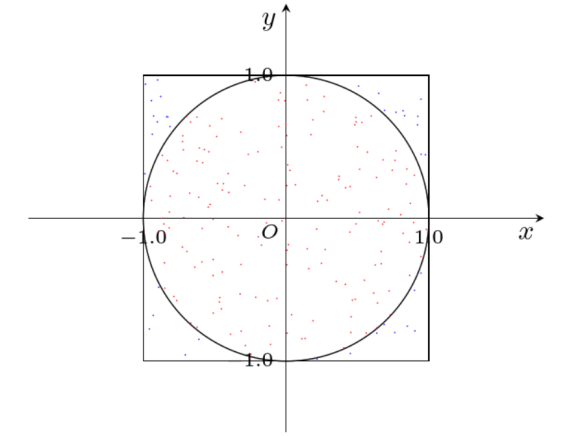
\includegraphics[width=0.5\linewidth]{soft/screenshot002}
	\caption{Illustration de l'estimation de $\pi$ par la méthode Monte-Carlo}
	\label{fig:screenshot002}
\end{figure}
Donc, la valeur approximative peut être calculée comme :
$$ \pi \approx 4 \times \dfrac{N_{cercle}}{N_{carre}}$$

\subsubsection{K-means}
K-means est un algorithme de clustering qui vise à partitionner un nombre de données en un nombre spécifié de clusters, en fonction de la proximité spatiale des valeurs moyennes. Il y a trois étapes principales :
\begin{enumerate}
\item Choisir arbitrairement K centres de clusters.
\item Calculer la distance entre chaque donnée et chaque centre, et assigner les données aux clusters adaptés.
\item Mettre à jour chaque centre selon la moyenne des données dans chaque cluster.
\end{enumerate}
On fait l’itération de ces trois étapes jusqu’à convergence. Mais en pratique, il est mieux de fixer le nombre des itérations afin de pouvoir converger en un temps constant. On commence le programme avec les données à 2 dimensions, après on l’optimise à dimension quelque afin de s’adapter aux datasets différents. Pour les tests sur PC, on fixe le nombre des itérations à 10.

\subsubsection{Analyse par Composantes Principales}
PCA est un algorithme d'apprentissage automatique qui est utilisé afin de réduire la dimensionnalité au sein d'un ensemble de données tout en conservant autant d'informations que possible. Cette action s'effectue en recherchant un nouvel ensemble de variables appelées composantes, qui constituent les composés des caractéristiques originales décorrélées les unes les autres. Les composants sont également contraints de telle sorte que le premier composant représente la plus grande variabilité possible dans les données, le deuxième composant la deuxième variabilité la plus importante, et ainsi de suite.

La représentation ci-dessous est un exemple d’application de l’algorithme afin de passer d’un espace 3D à un espace 2D:
\begin{figure}[H]
	\centering
	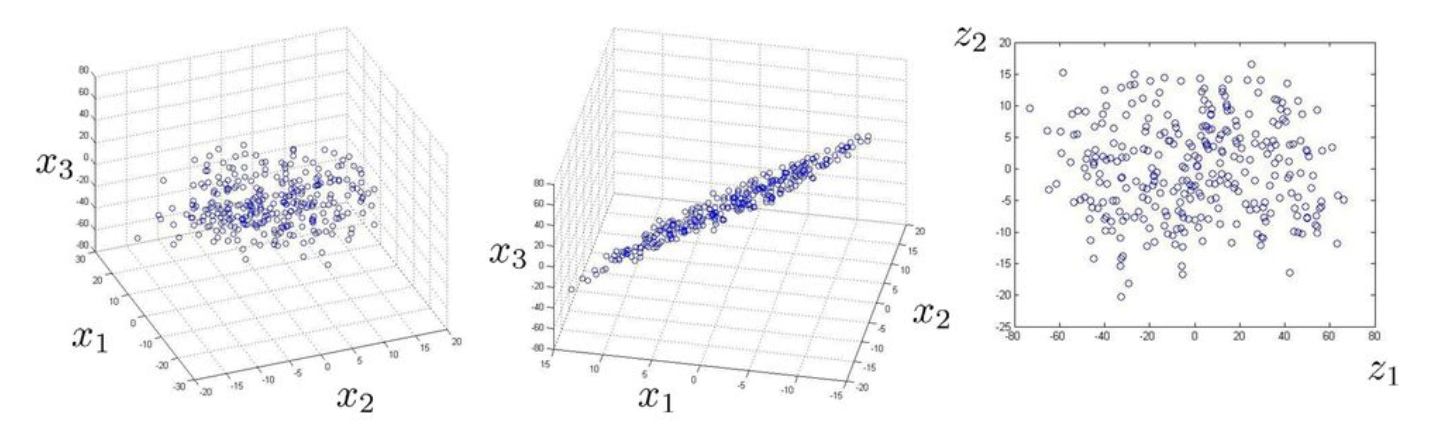
\includegraphics[width=0.8\linewidth]{soft/screenshot003}
	\caption{Représentation des projections de PCA}
	\label{fig:screenshot003}
\end{figure}
\subsubsection{Coefficient de Pearson}
La corrélation est une quantification de la relation linéaire entre des variables continues. Le calcul du coefficient de corrélation de Pearson repose sur le calcul de la covariance entre deux variables continues. 
Le coefficient de corrélation est ainsi exprimé de la manière suivante :
$$ r = \dfrac{Cov(X,Y)}{\sigma _X \sigma _Y}$$

Avec Cov(X,Y) la covariance entre les variables X et Y, et $\sigma _X$ et $\sigma _Y$ les écarts types respectifs de X et Y.L’algorithme a été testé avec plusieurs jeux de données avec un nombre d’observations allant de 10 à 20 pour deux variables.
\subsubsection{Décomposition par valeur singulière}
SVD est similaire à PCA.  Les deux algorithmes sont utilisés pour la réduction de la dimension de données. Mais avec SVD, on peut obtenir la décomposition de la matrice (données) dans deux directions. Il décompose une matrice A sous la forme suivante :
$$ A = U . \Sigma . V^T$$ 
avec :
\begin{itemize}
\item A: une matrice de dimension MxN
\item U : une matrice de dimension MxM, chaque colonne Ui est un vecteur propre de ($AA^T$)
\item $\Sigma$ : une matrice diagonale de dimension MxN, les éléments diagonaux sont $\sqrt (\lambda_i)$, avec $\lambda_i$ la valeur propre correspondante à $U_i$ . Les éléments sont dans l’ordre décroissant.
\item $V^T$: une matrice de dimension NxN, chaque ligne est un vecteur propre de ($A^TA$).
\end{itemize} 

\subsection{Implémentation et tests des algorithmes sur ARM}
Afin d'exécuter les algorithmes sur la carte Zynq, il faut configurer la carte comme le permettent les outils de Vivado. On ne détaillera pas ces configurations (en terme de zone mémoire attribué au code et aux données) sur ce rapport ni les binaires compilés obtenus.

\subsection{Optimisation des algorithmes sur ARM}
En général, il y a trois aspects qui seront pris en compte pour l’optimisation logicielle :
\begin{itemize}
\item Délais de branchement
\item Utilisation de cache
\item Dépendances de données
\end{itemize}
Maintenant, la plupart des optimisations sont effectuées par le compilateur avec différentes options. Ici pour GNU, il y a quatre niveaux d’optimisation :
\begin{itemize}
\item O0 : pas d’optimisation
\item O1 : l’optimisation par défaut, qui est faite sur les branchements et les constantes des grandes fonctions qui occupent beaucoup de mémoire
\item  O2 : l’optimisation au niveau du registre et de l’instruction 
\item O3 : l’optimisation en déroulant les boucles, utilisant la vectorisation SIMD, faisant \texttt{inline} les fonctions, mais prend plus de mémoire et de temps pendant la compilation
\item Os : l’optimisation sur la taille du code
\end{itemize}

Par exemple, BMM est déjà une optimisation pour calculer la multiplication des matrices. Si les blocs sont de taille suffisamment petite pour tenir entièrement dans le cache, il y aura d’échec de cache quelle que soit la méthode de multiplication.

On peut conclure que toutes les options d'optimisation (-O1, -O2, -O3, -Os) par le compilateur peuvent réduire considérablement le temps d'exécution. En comparant la taille du code (segment “text”) après les différentes optimisations, on peut voir que la taille du code sera toujours la plus petite si l’on choisit l’option “-Os” qui est spéciale pour l’optimisation de taille. En plus avec “-O3”, la taille du code sera plus longue par rapport à d'autres options même si son niveau d’optimisation est le plus haut.

\subsection{Implémentation sur $\mu$blaze}
Les processeurs Hardcore ont de bonnes performances, mais ne peuvent être utilisés que dans des cartes spécifiques. Les processeurs Softcore (par exemple MicroBlaze ici), en revanche, ont de faibles performances, mais sont très portables sur FPGA.

Le MicroBlaze est un microprocesseur softcore RISC, d'architecture Harvard, entièrement 32 bits. Il présente ainsi 32 registres internes de 32 bits, des bus instructions et données internes, et externes.
Le processeur possède 70 options de configuration, parmi lesquelles on trouve : un pipeline (3 ou 5 niveaux), opérateur de division, de décalage, FPU, logique de débug, mémoires cache instructions et données.

L’architecture du cœur Microblaze est représentée par la figure \ref{fig:screenshot004} :
\begin{figure}[H]
	\centering
	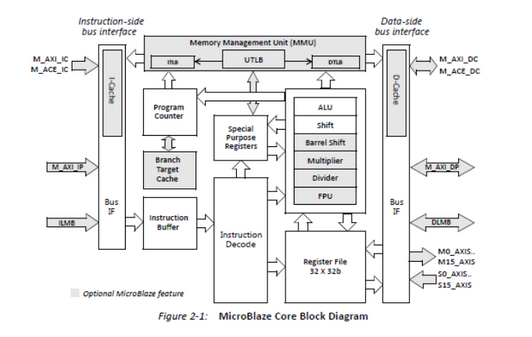
\includegraphics[trim= 0  20 0 0,clip,width=0.8\linewidth]{soft/screenshot004}
	\caption{Schéma bloc de l'architecture du $\mu$blaze}
	\label{fig:screenshot004}
\end{figure}


\section{Conception Synthèse Haut Niveau}
Cette conception dite HLS consiste à convertir un code C/C++ en une implémentation RTL d'un code VHDL ou Verilog. La difficulté de cette étape est de comprendre que tout ce qui est en C/C++ n'est pas forcement implémentable ou mal effectué par le trans-compilateur. En effet, on tente de passer d'un schéma de flot de contrôle vers un schéma de flot de données. Par exemple, le fonctions récursives sont simplement impossibles à implémenter matériellement. Certains algorithmes itératif à critères d'arrêt dynamique doivent subir une reconversion. Au final, le but est de générer une IP matérielle dite HLS et quelle soit implémentable par l'équipe gérant le matériel.

Dans cette partie, on présente le principe dernière l'outil HLS et quelques-unes des optimisations qu'il propose. Mais aussi, expliquera le raisonnement derrière l'approche de la génération matériellement automatisée.

\subsection{Conception d'une IP avec directives}
Une IP sera encapsulée en elle-même. Ce qui fait que l'implémentation matérielle n'aura aucun contrôle sur ce qui se passe dans l'IP.
Afin de pouvoir optimiser l'IP HLS créée, il faut dans un premier temps faire une analyse des dépendances pendant l'exécution de l'algorithme. Cette analyse est faite en 2 temps: 
\begin{itemize}
\item En premier, automatiquement par Vivado HLS qui possède des outils permettant de détecter des dépendances, d'essayer de les corriger/éliminer ou de suggérer à l'utilisateur d'utiliser les directives proposées.
\item En second, l'utilisateur, à l'aide des directives HLS, modifie la synthèse sans modifier le code lui même.
\end{itemize}
 Les directives les plus intéressantes, pour les algorithmes demandant plusieurs itérations et ayant une implémentation séquentielle tel que Kmeans, sont \texttt{FLATTEN}, \texttt{PIPELINE} et \texttt{UNROLL}.
 
\paragraph{Flatten} : Elle consiste à essayer de simplement aplatir la boucle en la rendant en une simple suite d'instructions. Ceci permettra de concevoir un flot de donnée matériel en RTL. Cette directive n'est possible que si toutes les boucles internes peuvent être aplaties et donc qu'il n'y ait pas de dépendances en données.
\paragraph{Pipeline} : Applicable aux boucles, fonctions et opérateurs, cette directive divise les opérations en plusieurs étages successifs de conception simple qui à chaque cycle effectuent une opération en 1 cycle. Le pipeline est très efficace pour diminuer la latence des opérateurs mais occupe une plus grande surface sur le FPGA contrairement à une version multi-cycles. Deux aspects important du pipeline sont : son intervalle d'initialisation (II) qui représente le nombre de cycles après lequel le pipeline peut consommer une donnée; et la latence i.e. le retard à la sortie.

\paragraph{Unroll} : Quand un calcul dans une boucle possède des dépendances de données et une latence plus grande que la durée d'une itération, il est conseillé de dérouler la boucle d'un facteur. par exemple au lieu de traiter les données 1 à 1, on peut traiter n à n. Cette directive peut occuper beaucoup plus de surface FPGA. Il faut donc l'utiliser uniquement quand le nombre d'itération est faible.

Une fois un opérateur/fonction optimisé(e), il faut analyser le nombre d'accès mémoire qu'il effectue en lecture/écriture. Si une mémoire ne fournit qu'un port d'accès, une seule lecture/écriture peut être fait en même temps dans le même cycle (en prenant en compte que la lecture prend deux cycles selon HLS). Il existe plusieurs stratagèmes pour contrer cela. HLS propose \footnote{\href{https://japan.xilinx.com/html\_docs/xilinx2017\_4/sdaccel\_doc/okr1504034364623.html}{Xilinx Pragma}} :
\paragraph{Map} : Permet d'agréger différents blocs mémoires en un seul afin de réduire l'usage des ressources RAM.
\paragraph{Partition} : Au contraire, cette directive permet de diviser un tableau en plusieurs sous tableau et donc blocs mémoires voir même registre afin d'augmenter le débit lecture/écriture au prix d'une coût matériel plus élevé.
\paragraph{Reshape} : Permet de redimensionner un bloc mémoire d'un certain facteur de manière entier ou cyclique afin d'avoir un bon compromis entre les deux directives précédentes. Celui-ci est le plus souvent utiliser car il permet d'avoir plusieurs accès mémoire matériels en fonction du nombre de circuits concurrents désirant d'accéder à la même donnée.

\subsection{Interfaçage d'une IP avec Axi/Axilite}
Il est possible d'interfacer une IP matériellement grâce à une panoplie de pointeurs bas niveau. Cette démarche permet d'avoir un contrôle très fin sur les adresses auxquelles le matériel accèdent. Mais par contre, complexifie tellement la gestion matérielle qu'elle devient très chronophage voir impossible pour un humain. Il est donc nécessaire de d'utiliser les interfaces fournis par Xilinx pour la carte ZedBoard, les \textit{Axi} et \textit{Axilite}. Il suffit de définir les ports entrées/sorties de l'IP HLS en tant que maître dans un port Axi et leur données une profondeur (la longueur de la mémoire FIFO). Aussi, il faut définir la fonction \textit{Top-level} comme étant apte à contrôler le bus et donc à recevoir les signaux de synchronisation depuis un CPU (soft ou hard) via l'interface \textit{Axilite}.

Dans les faits, On copie les entrées depuis l'interface du Axi dans des blocs mémoires locaux. Ceci fait que HLS infère des copies en rafale à la place de \textit{memcpy}.Donc, on travaille sur des pointeurs locaux puis on exporte le résultat par Axi output. Il ya donc une abstraction totale de l'interaction mémoire entre une IP HLS et le reste de l'architecture.

\subsection{Approche d'implémentation des algorithmes}
Afin de pourvoir transcrire les algorithmes discutés avec l'équipe logicielle, il d'abord effectuer une analyse de faisabilité en HLS. Car, on ne synthétise  pas un algorithme qui ne vaut pas le coût d'être accéléré. Ensuite, on procède à une analyse des besoins matériels pour en déduire les points d'apparition de goulots. Choisir entre la réinterprétation de l'algorithme ou la fragmentation en sous-opérateurs. 

Dans la première, on doit réétudier le processus de l'algorithme. Puis, décider si celui-ci est modifiable sans corrompre les résultats ou bien possède une autre implémentation qui puisse satisfaire au mieux les contraintes matérielles. Deux exemples : l'estimation du nombre $\pi$ par la méthode Monte-Carlo qui ne peut être effectué simplement car la fonction \texttt{rand()} n'existe pas en matériel. Il faut alors concevoir un générateur de nombre aléatoire matériel qu'il soit à base d'oscillateur en anneau ou autre. Un deuxième exemple est de modifier le critère d'arrêt de K-means i.e. changer la boucle \texttt{while} qui est d'une durée d'exécution indéterminé en boucle \texttt{for} qui elle est finie en terme de nombre d'itérations. Plusieurs autres optimisations sont faisables mais il n'y a pas de règles évidentes pour ceci. Il faut soit mener des recherches sur la documentation et les forums ou se fier à son intuition et expérience.

Dans la fragmentation en sous-opérateurs, si un algorithme a des parties non dissociables, donc dépendantes au sein d'une boucle, on peut imaginer à le séparer en sous-opérateurs afin d'optimiser ces entités là. Ceci peut offrir un grand gain en performance temporelle mais a deux inconvénients majeurs : Plus de surface par opérateur sera requis à cause de l'implémentation de blocs mémoires "dupliqués" et elle nécessite que la partie développement matériel écrive un protocole d'appel de l'IP plus complexe à développer. Après plusieurs tests, on estime que cette méthode d'optimisation ne sera pas utilisée à cause de contraintes temporelles.

\subsubsection{Critères de conception d'IP}
Il existe un nombre assez élevé d'optimisation effectuées automatiquement ou manuellement par le logiciel HLS. Un premier facteur limitant lors de la conception est la surface FPGA occupée par l'IP (éléments logiques,DSP,...). Il est simplement impossible d'implémenter une IP qui ne peut pas être portée sur la carte. Donc, il faut limiter l'usage des directive \texttt{pipeline} et \texttt{unroll} mais aussi les blocs RAM internes. Le \textit{pipeline} possède un critère important qui est l'intervalle d'initialisation. i.e. combien de cycles il y a entre la consommation d'une donnée. Celui-ci est limité par les load/store comem on eput le voir sur la figure \ref{fig:scheduler}, load prend 2 cycles et donc le pipeline est bloqué pend cela. il est difficile de masqué ces chargements et comme pour un CPU, on doit payer le prix soit en temps soi ou bien  en surface FPGA.

\begin{figure}[H]
	\centering
\begin{subfigure}{.75\textwidth}
	\centering
	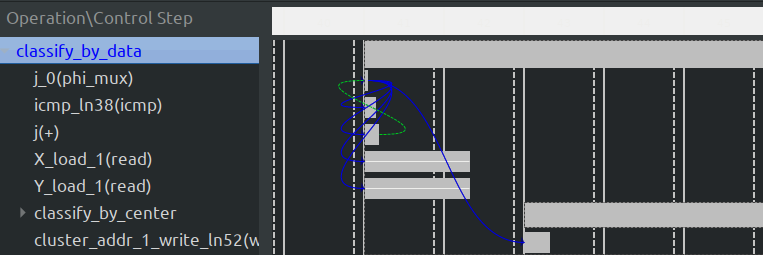
\includegraphics[height=4cm]{hls_fig/screenshot005}
	\caption{Ordonnancement temporel d'une boucle dans une IP}
	\label{fig:scheduler}
\end{subfigure}
\begin{subfigure}{.20\textwidth}
	\centering
	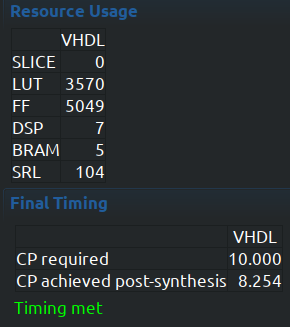
\includegraphics[height=4cm]{hls_fig/screenshot004}
	\caption{Implémentation}
	\label{fig:timing_met}
\end{subfigure}
\caption{Conception de l'IP :}
\end{figure}

Le deuxième paramètre limitant l'implémentation de l'IP est la fréquence de fonctionnement. HLS prend une période (donc fréquence) objective et "essayera" de synthétiser l'IP demandée à cette fréquence. Il est possible de le forcer à relaxer la synthèse afin de respecter ce critère.

Une solution possible à cette contrainte est d'utiliser des horloges différentes sur la carte qui ce soit par le Zynq ou le \texttt{SmartClock} (voir \ref{SmartClock}). Les algorithmes SVD et PCA ne sont pas implémentées à cause de la présence de plusieurs séquences de contrôle durs à optimiser dans les contraintes temporelles données. Il est aussi important de noter qu'une IP agit comme un accélérateur matériel non-bloquant pour le CPU. i.e. le CPU est libre pendant tout le temps d'exécution.

La figure \ref{fig-hls} montre un résumé de quelques IPs implémentées. Toutes les IP ont pour période de fonctionnement objective : \textbf{10} ns. La figure \ref{fig:timing_met} indique que l'Ip a était synthétisée avec succès et qu'elle respecte les contraintes temporelles imposées.

\begin{figure}[H]
	\centering
	\begin{subfigure}[H]{.31\linewidth}
		\centering
		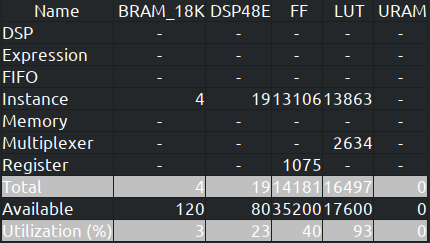
\includegraphics[width=\linewidth]{hls_fig/screenshot001}
		\caption{Pearson}
	\end{subfigure}
	\begin{subfigure}[H]{.31\linewidth}
		\centering
		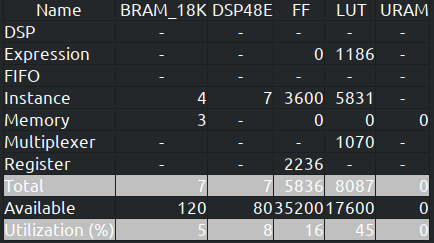
\includegraphics[width=\linewidth]{hls_fig/screenshot002}
		\caption{Kmeans}
	\end{subfigure}
	\begin{subfigure}[H]{.31\linewidth}
		\centering
		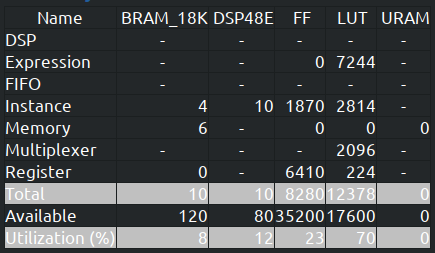
\includegraphics[width=\linewidth]{hls_fig/screenshot003}
		\caption{Matrix Block Mult.}
	\end{subfigure}	
	\caption{Occupation des ressources FPGA pour différentes IP}
	\label{fig-hls}
\end{figure}

\section{Implémentation matérielle}
\subsection{Introduction}
Tout l'objet de cette partie est de concevoir une design à l'aide de Vivado pour exécuter les calculs de la partie Software. Elle doit fournir des exemple de matériel pour qu'ils test leur logiciel et est aidée par la partie HLS pour accélérer les calculs. La finalité des design est de permettre d'embarquer les calculs ainsi accélérés pour une utilisation sur par exemple du matériel roulant.
\subsection{Demo multi-CPU}
Une première démo a été conçu pendant le développement des algorithmes jusqu'à l'arrivée des IP HLS. On profite ainsi de l'absence de dépendance avec les autres parties pour explorer des architecture de système.
\subsubsection{Concept et problem}
Ce design Multi-CPU se propose de juxtaposer aux 2 processeurs ARM embarqués dans le \textit{Zynq}, un softcore \textit{microblaze} implémenté dans la logic programmable (PL/FPGA). L'idée étant de faire tourner des codes sur les 2 processeurs ou d'utiliser le \textit{microblaze} pour du contrôle en utilisant les interruptions.


Un premier design a été réalisé:
\begin{figure}[H]
	\centering
	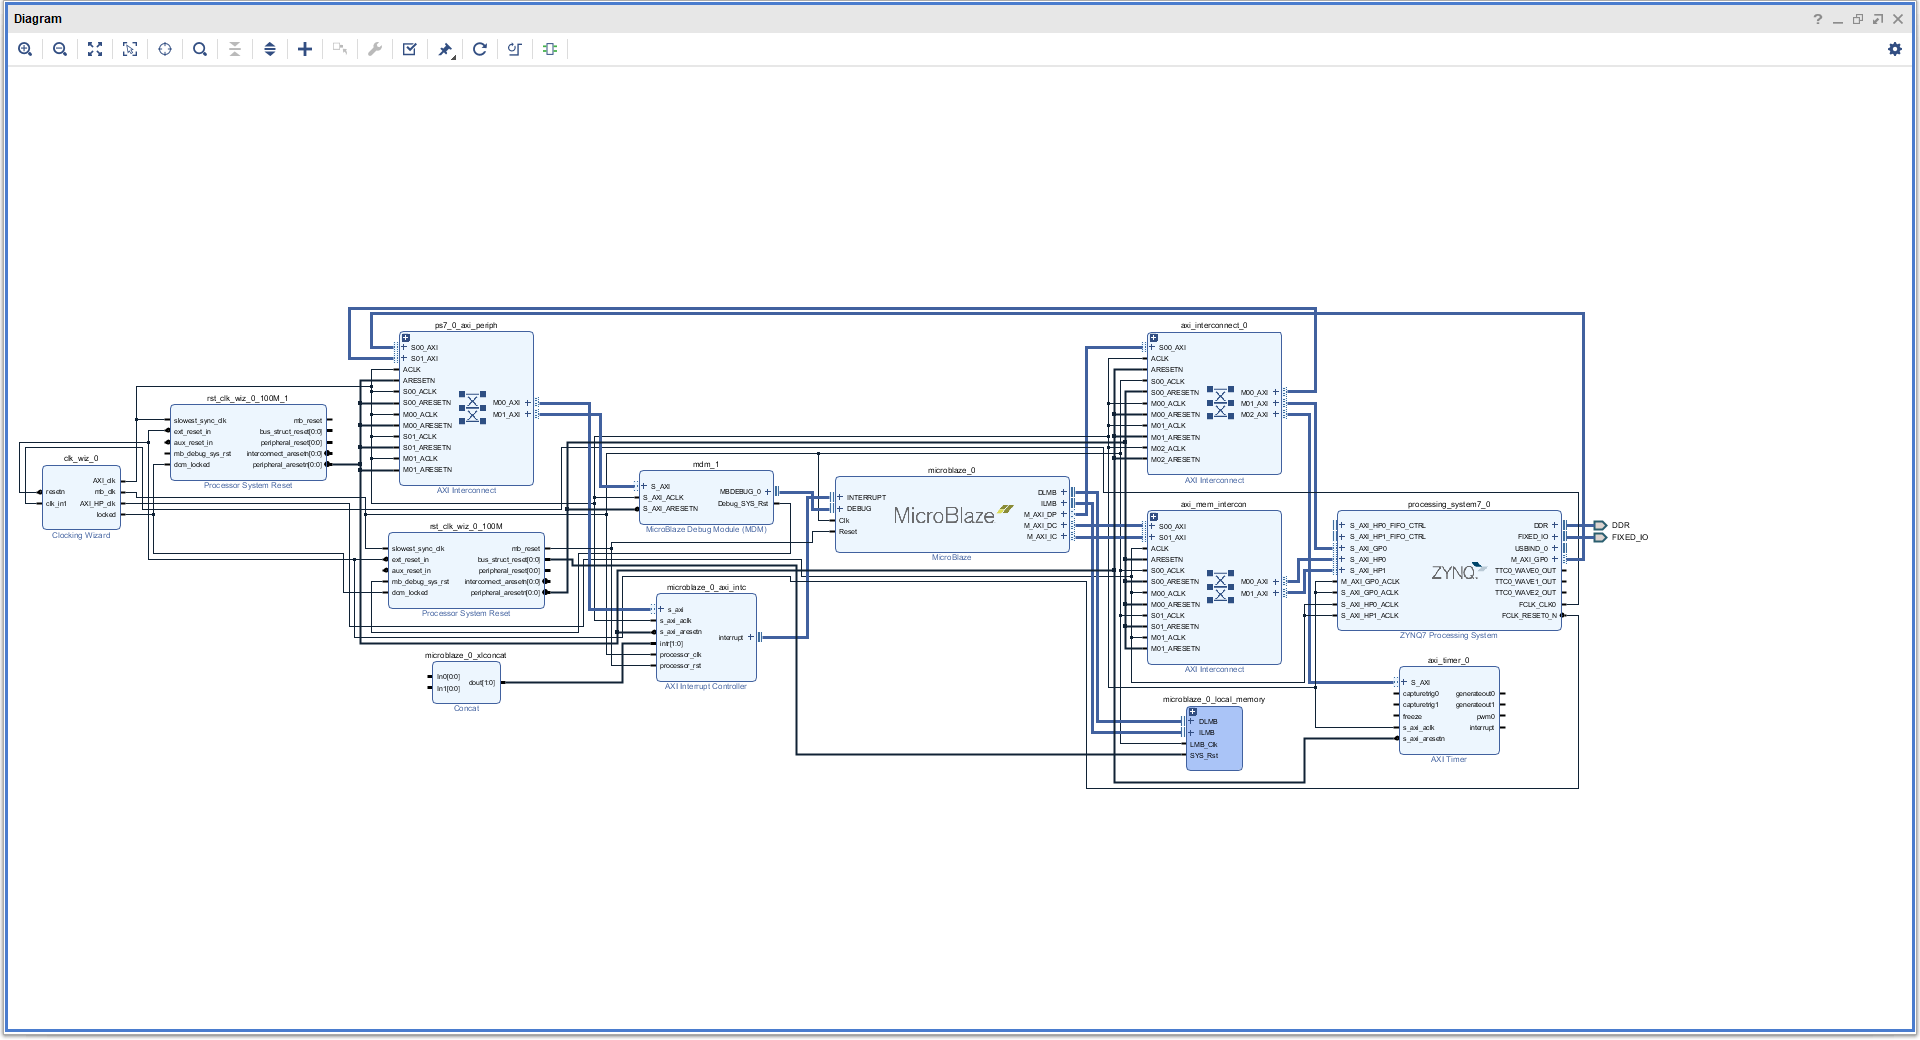
\includegraphics[width=\linewidth]{im/mb1.png}	
	\caption{Exemple de design pour le Multi CPU pouvant exécuter un programme sur le FPGA et sur le microblaze. }
	\label{fig-mb}
\end{figure}

Maintenant que le microblaze est rajouté, il peut être intéressant de pouvoir lui passer des données. Le microblaze est déja connecté à la RAM du ZYNQ. Donc en théorie, il peut déjà recevoir et envoyer des donnés. On peut déjà les faire s'exécuter tous les 2 depuis la RAM du ZYNQ (cela permet d'agrandir le heap et le stack pour éviter les dépassement).
\begin{figure}[H]
	\centering
	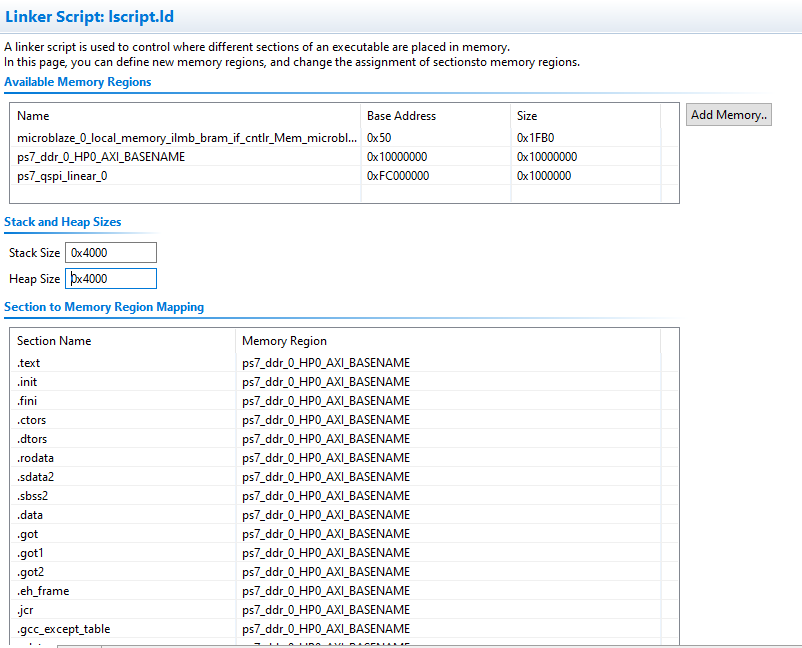
\includegraphics[width=\linewidth]{im/mb2.png}	
	\caption{Linker script du microblaze : exécution depuis la DDR et stack et heap étendus}
	\label{fig-link}
\end{figure}

Une des choses que l'on voudrait pouvoir faire est de passer une grande quantité de données et des instructions au microblaze. Du fait qu'il a accès à la RAM du \textit{Zynq}, il faudrait juste pouvoir lui envoyer des instructions. Si possible dans un emplacement fixe de la mémoire.

\subsubsection{Utilisation de la BRAM}
Pour passer des instructions du \textit{Zynq} au \textit{microblaze}, On décide d'utiliser les BRAM. On crée ainsi un block design qui a en plus du lien avec la DDR du \textit{Zynq}, a aussi des BRAMs. A l'intérieur de celles-ci, on pourra placer des adresses pour les données et des instructions sur ce qu'il faudra en faire.

\begin{figure}[H]
	\centering
	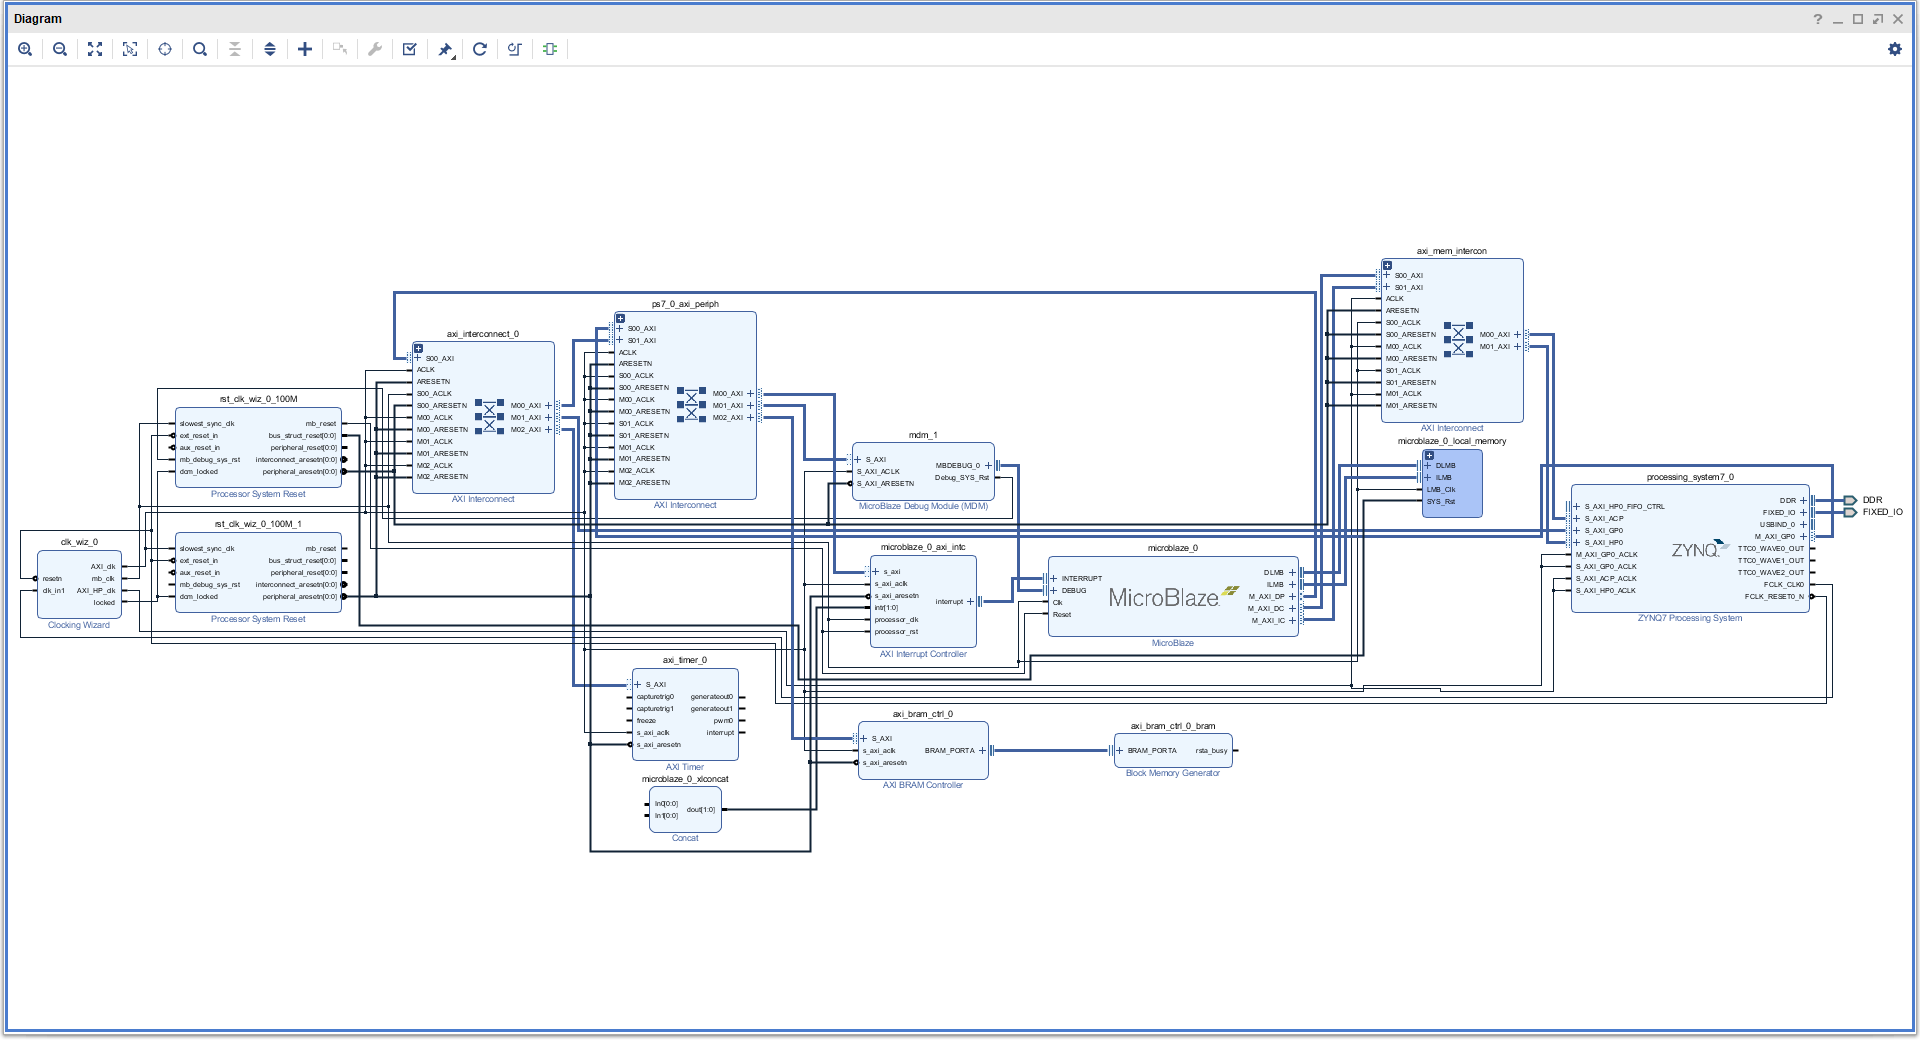
\includegraphics[width=\linewidth]{im/bram1.png}	
	\caption{Block design pour tester la BRAM :}
	\label{fig-bram1}
\end{figure}


\subsubsection{Passage de données vers un microblaze}
Une fois cela fait, on a développé 2 applications : une pour le \textit{Zynq} et une pour le \textit{microblaze}.



\begin{figure}[H]
	\begin{multicols}{2}
		\begin{lstlisting}[language=C]
		
		int main()
		{
		XTime Start_Time, End_Time;
		
		init_platform();
		
		print("Zynq:Hello World\n\r");
		XTime_GetTime((XTime *) &Start_Time);
		char * test =(char*)XPAR_AXI_BRAM_CTRL_0_S_AXI_BASEADDR;
		
		memcpy(test,"un message\n",20);
		
		while(1){
		XTime_GetTime((XTime *) &End_Time);
		sprintf(test,"message à %lli",(End_Time - Start_Time));
		sleep(1);
		}
		\end{lstlisting}	
		\bigskip
		\begin{lstlisting}[language=C]
		int main()
		{
		char* test=(char*)XPAR_AXI_BRAM_CTRL_0_S_AXI_BASEADDR;
		init_platform();
		
		print("micro:Hello World 2\n\r");
		sleep(10);
		
		
		
		while(1){
		printf("micro:%s\n",test);
		sleep(1);
		}
		}
		
		\end{lstlisting}	
	\end{multicols}		
	\caption{Code du microblaze(droite) et du zynq(gauche) pour l'envoie et la réception de message}
\end{figure}
On peut ainsi facilement passer des adresses du Zynq au microblaze grâce à la BRAM.La finalité de ce design a été de permettre à l'équipe logicielle de tester leur programme sur la carte. La figure \ref{fig-bram2} montre l'exécution du codes.
\begin{figure}[H]
	\centering
	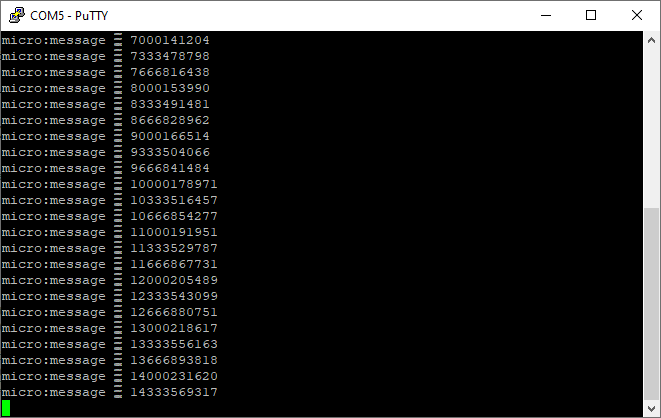
\includegraphics[width=\linewidth]{im/bram2.png}	
	\caption{Démonstration de la BRAM : le microblaze affiche un message envoyé depuis le Zynq}
	\label{fig-bram2}
\end{figure}

\subsection{IP HLS}
Dès que la première IP HLS a été finalisée, il a été question de les intégrer dans un design. Donc, un design a été conçu pour les tester.
\subsubsection{Concept}
Pour accélérer, les programmes que l'on fait tourner sur les \textit{Zynq}, la partie HLS à réaliser des accélérateurs matériels à l'aide des outils \textit{Xilinx}. Ces accélérateurs se présentent comme des IP que l'on peut rajouter dans un bloc design. Il faudra envoyer des donnés à ces IP pour quelle fasse les calculs à la place du \textit{Zynq} : Beaucoup plus rapidement mais aussi non bloquant pour le CPU.

Ces IP sont commandées par le \textit{Zynq} qui leur donne également des emplacements mémoires comme paramètres. Elles disposent d'accès directe à la mémoire DDR du \textit{Zynq} pour pouvoir charger localement les données et ranger les résultats.

\subsubsection{Implémentation et clocking}
Une fois les IP mises dans un répertoire communs et que ce répertoire est signalé à \textit{ Vivado} comme contenant des IPs, On peut les utiliser dans un block design classique.
\paragraph{Relier les IPs au Zynq}
Les IPs HLS se présentent comme suivant:
\begin{figure}[H]
	\centering
	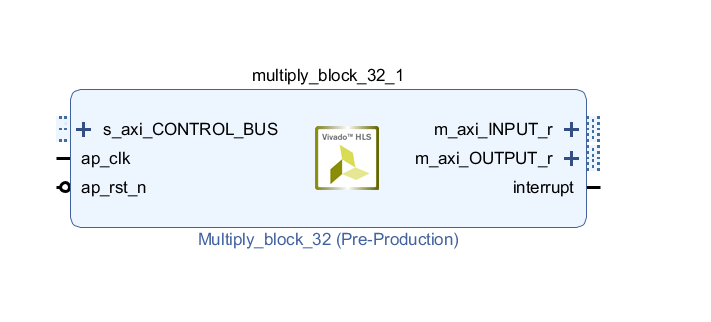
\includegraphics[width=\linewidth,trim=0 50 0 50,clip]{im/ip1.png}	
	\caption{Exemple d'IP avec ses différents ports}
	\label{fig-ip1}
\end{figure}

Elles ont 6 ports: 
\begin{itemize}
	\item[•]Un Port Slave AXILite appelé \lstinline[language=bash]{CONTROL_BUS} qui sert a commandé l'IP.
	\item[•]2 Ports Master AXI appelés \lstinline[language=bash]{INPUT} et \lstinline[language=bash]{OUTPUT} qui servent à l'IP pour accéder à des données en mémoire.
	\item[•] Des ports \lstinline[language=bash]{clk} et \lstinline[language=bash]{rst} qui permettent à l'IP d'avoir une clock indépendante (on utilisera cela pour avoir de meilleures performances)
	\item[•]Un port \lstinline[language=bash]{interrupt} qui n'as pas été utilisé mais pourrait l'être utilisé avec un microblaze pour déclencher une interruption dès que l'IP finit.
	
\end{itemize}

On relie cette IP au Zynq de la manière suivante:
\begin{itemize}
	\item[•]Les ports \lstinline[language=bash]{INPUT} et \lstinline[language=bash]{OUTPUT} sont reliés au Slave ACP du ZYNQ pour pouvoir accéder à ces mémoires et avoir la cohérence des caches.(figure \ref{fig-acp}).
	\item[•] On relie les ports \lstinline[language=bash]{CONTROL_BUS} au Master GP du Zynq pour pouvoir envoyer des commandes (les commandes étant moins critiques, elles ne passent pas par les interfaces rapides )
\end{itemize}


\begin{figure}[H]
	\centering
	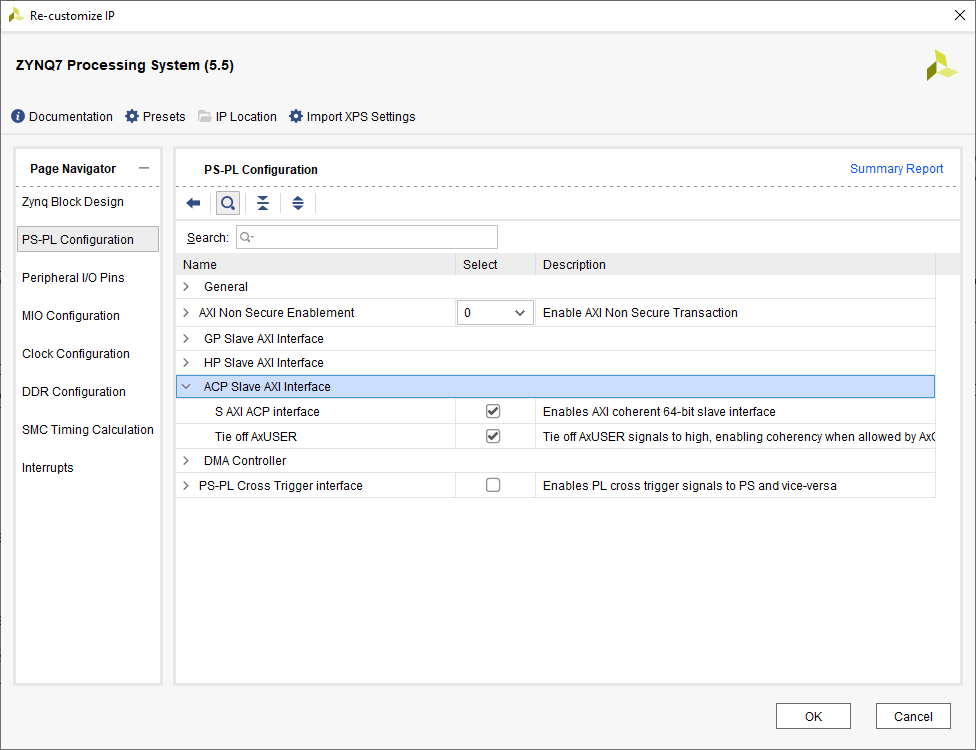
\includegraphics[width=\linewidth]{im/ip2.png}	
	\caption{Paramètre du Zynq: ce qu'il faut cocher pour avoir l'interface ACP et la cohérence des caches}
	\label{fig-acp}
\end{figure}

\begin{figure}[H]
	\centering
	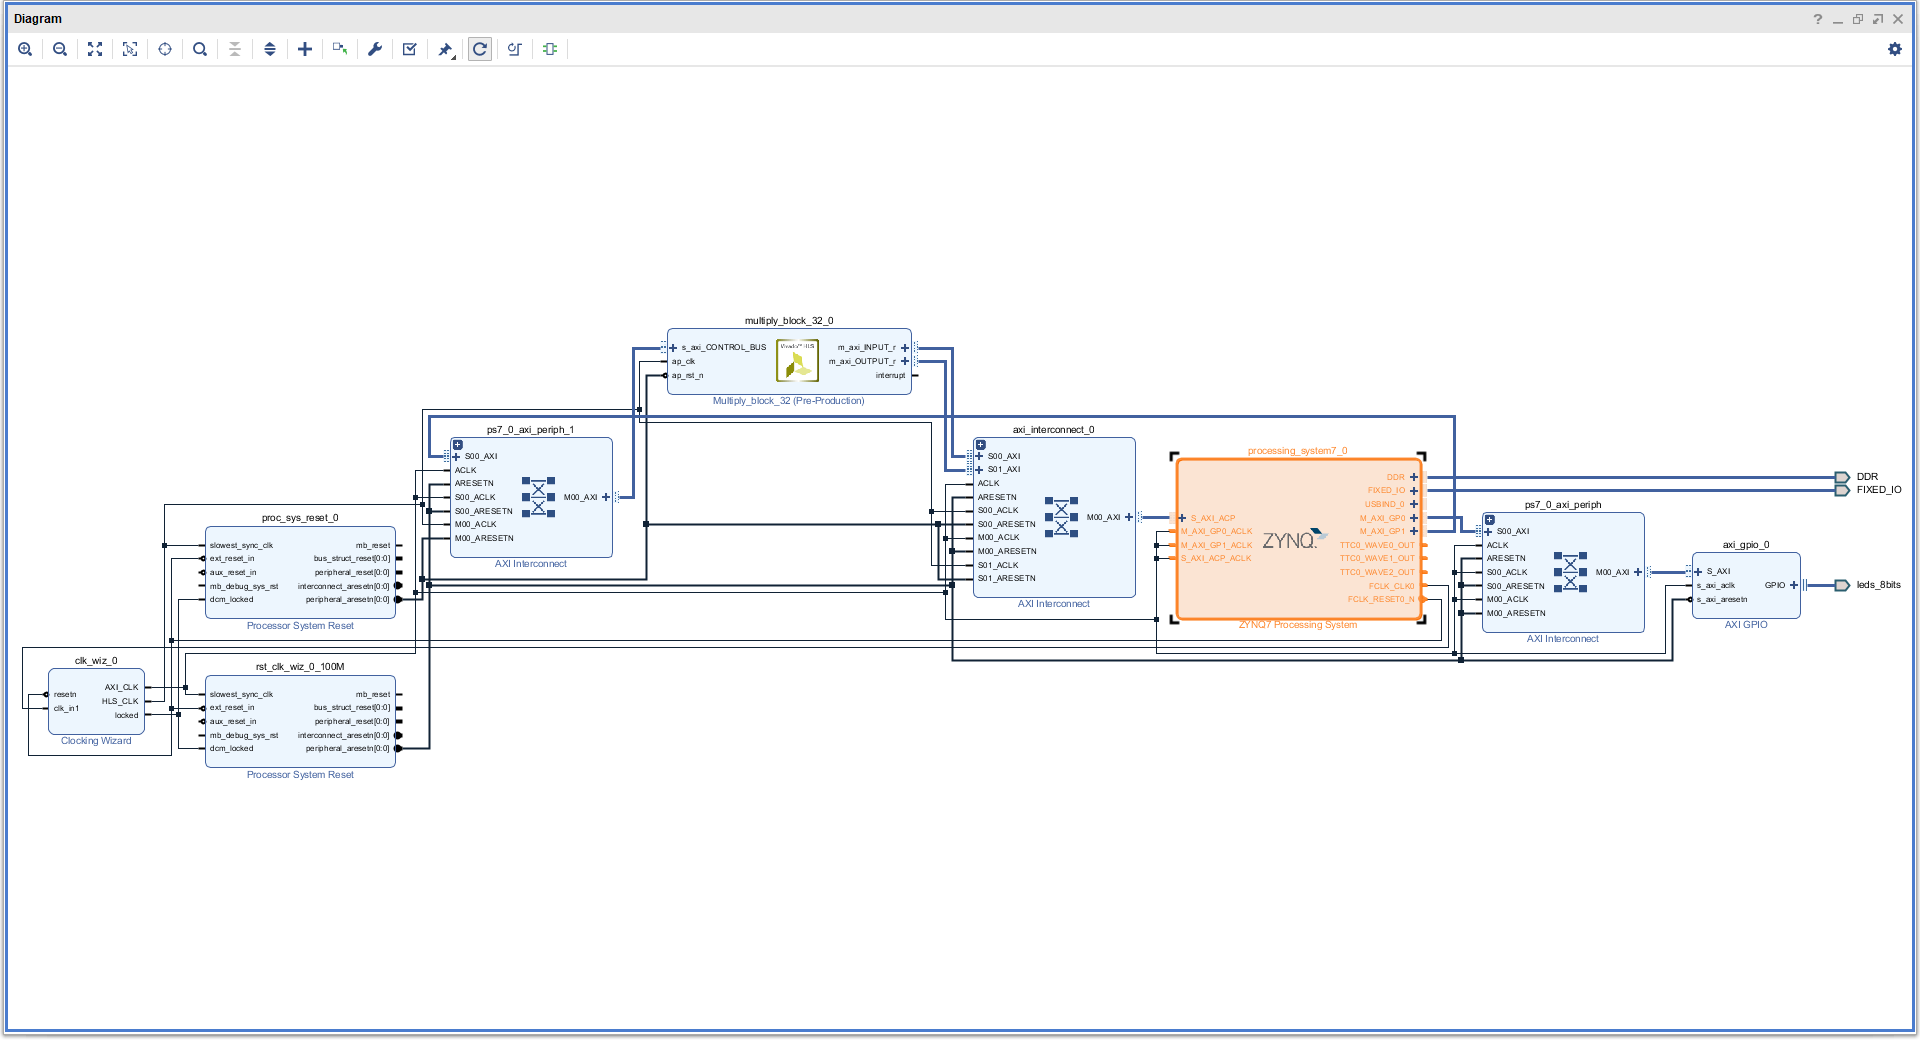
\includegraphics[width=\linewidth]{im/ip3.png}	
	\caption{Exemple de design pour l'IP multiply\_block\_32}
	\label{fig-ip}
\end{figure}

On a fait en sorte dans le bock design que les clocks des IP et la clock du HLS soit indépendantes. Cela permettra de tiré le plus de performance des IP plus tard.


\paragraph{Fonction pour le SDK}
A partir de là, après synthèse, placement et routage du design, on dispose d'un entête spécial par exemple:
\begin{lstlisting}[language=C]
#include "xmultiply_block_64.h"
\end{lstlisting}
qui va permettre d'interagir simplement avec une IPS HLS.

Ainsi le code suivant contient 2 fonctions qui permettent d'initialiser une IP HLS(ici \textit{mul64}) et de l'utiliser pour faire un calcul.
\begin{lstlisting}[language=C]
//fonction d'initilisation de L'IP
void init_multiply_block_ip(XMultiply_block_64* mb,XMultiply_block_64_Config* mb_c){
int status=XMultiply_block_64_CfgInitialize(mb,mb_c);
XMultiply_block_64_DisableAutoRestart(mb);
XMultiply_block_64_InterruptGlobalDisable(mb);
XMultiply_block_64_InterruptDisable(mb, 1);
if(status!=XST_SUCCESS){
printf("Multiply Block: init_failed \r\n");
}
printf("idle=%lx,ready=%lx,done=%lx\n",XMultiply_block_64_IsIdle(mb),XMultiply_block_64_IsReady(mb),XMultiply_block_64_IsDone(mb));
printf("succes\n");
}

//fonction de lancement du calcul sur l'IP
void multiply_block_hw_call(XMultiply_block_64* mb_p,float* mA, float* mB, float* result){

//on charge les adresse des données et les sorties
XMultiply_block_64_Set_in_mA(mb_p, (u32)mA);
XMultiply_block_64_Set_in_mB(mb_p, (u32)mB);
XMultiply_block_64_Set_out_mC(mb_p, (u32)result);

//on attend d'être prêts.
while(!XMultiply_block_64_IsReady(mb_p));

//on lance
XMultiply_block_64_Start(mb_p);

//on attend d'avoir fini	
while(!XMultiply_block_64_IsDone(mb_p)){

}
//les résultat sont déja rangé donc on a fini.
return;

}

\end{lstlisting}
Grâce à l'utilisation des interfaces ACP et du fait qu'on ait activé le "\textit{tie off AxUser}", nous n'avons pas besoin de vider le cache puisque la cohérence est maintenue à travers l'AXI et malgré les modifications des données faites par l'IP.

\label{SmartClock}
\paragraph{Optimisation des clock avec les Timings}
On peut maintenant chercher à avoir le plus de performances possible avec nos IPs. Pour cela on va utiliser le fait qu'elles aient des clocks indépendantes de celle de l'AXI. On peut ainsi changer leur fréquence séparément du reste du système.

Grâce au \textit{timing report}, on peut connaître après implémentation quelle est la marge que l'on a par rapport au temps critique fixé par la clock. On peut ainsi corriger cette clock itérativement pour aller jusqu'au moment où l'on n'a plus aucune marge.

On a put par exemple monter la clock de l'IP \textit{mul64} de 100 à 130 MHZ.

\begin{figure}[H]
	\centering
	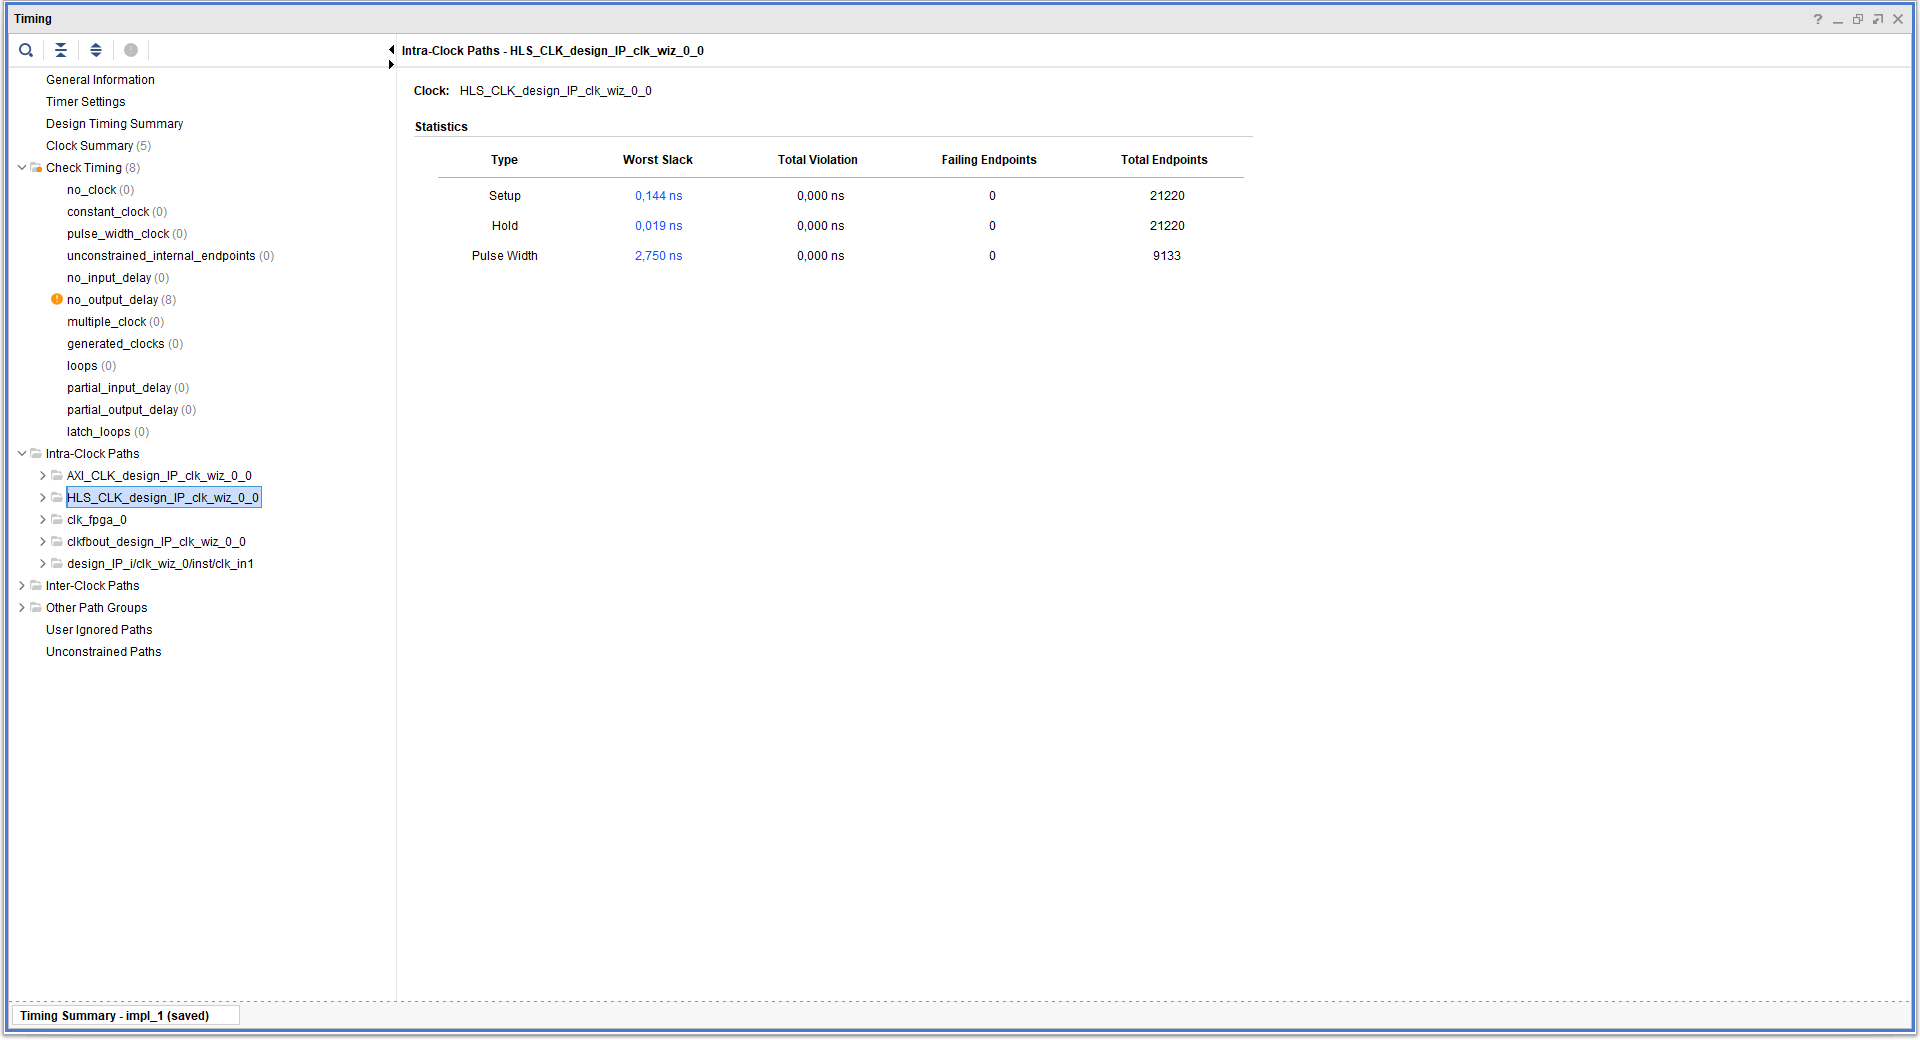
\includegraphics[width=\linewidth,trim= 0 300 500 0,clip]{im/timing.png}	
	\caption{Écran du timing report permettant de connaître le clock skew}
	\label{fig-clk}
\end{figure}

\subsubsection{Performances}
\subsection{Amélioration et future design}
Il s'agirait ensuite de construire un design utilisant et les IP et le \textit{microblaze} pour pouvoir, par exemple utiliser l'IP HLS de block matrix multiplication. Pour faire des multiplication de matrice plus grande en utilisant plusieurs fois l'IP sans avoir besoin de monopoliser le \textit{Zynq}, utilisant ainsi les interruption sur le \textit{microblaze.}

%exemple d'achitecture en cours de developemnt mais qui n'as pas put être fini.


\section{Performances Mesurées}
Dans cette section, on présente les résultats obtenu et validé pour les exécution sur PC standard, ARM, ARM+HLS et $\mu$blaze.
\subsection{Performances ARM}
L'exécution sur ARM donne les résultats montré en figure \ref{fig:screenshot005}. On retrouve bien la complexité algorithmique théoriques et que ces algorithmes sont proportionnels à la taille des données sauf pour Bloc-Matrix-Multiplication. qui lui dépend du formatage et du parcours (ijk) de ces données.
\begin{figure}[H]
	\centering
	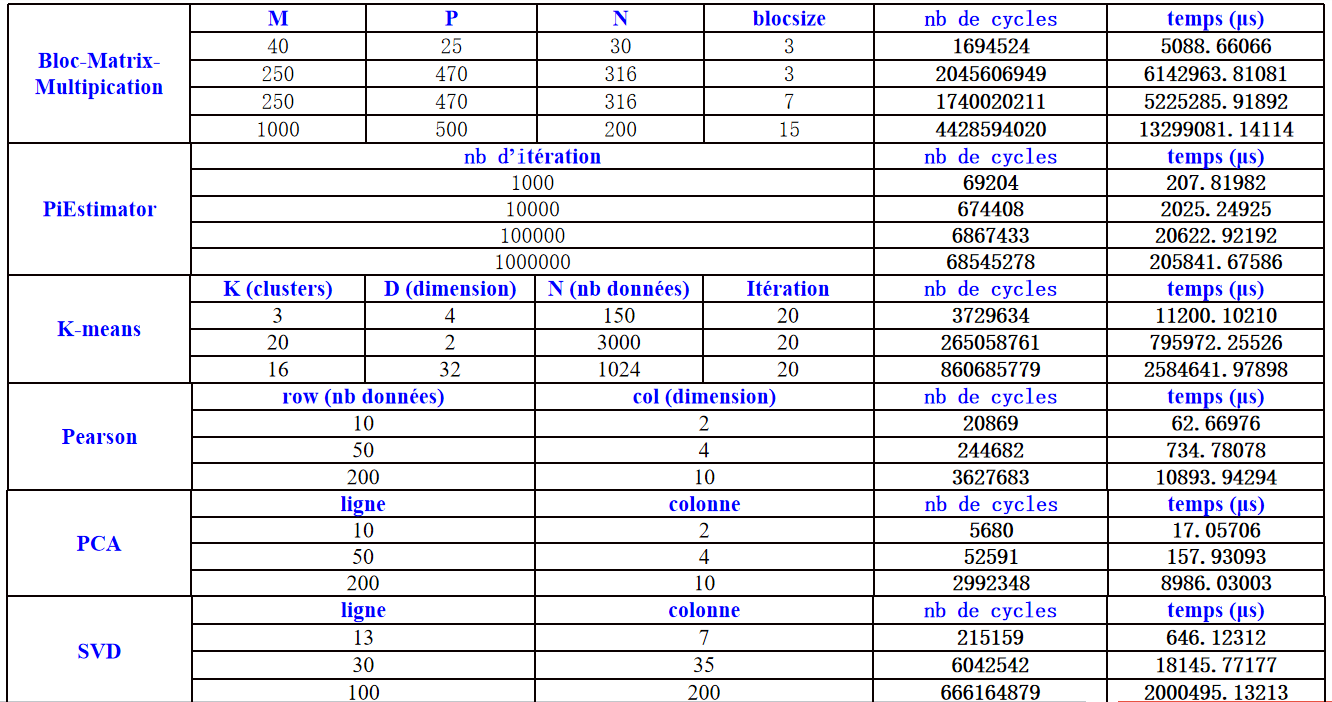
\includegraphics[width=\linewidth]{soft/screenshot005}
	\caption {Temps d'exécution sur ARM des différents algorithmes}
	\label{fig:screenshot005}
\end{figure}
On voit aussi le lien entre optimisations de compilation et performance en terme de taille de code et temps sur la figure \ref{fig:screenshot006} et \ref{fig:screenshot007}.
\begin{figure}[H]
	\centering
	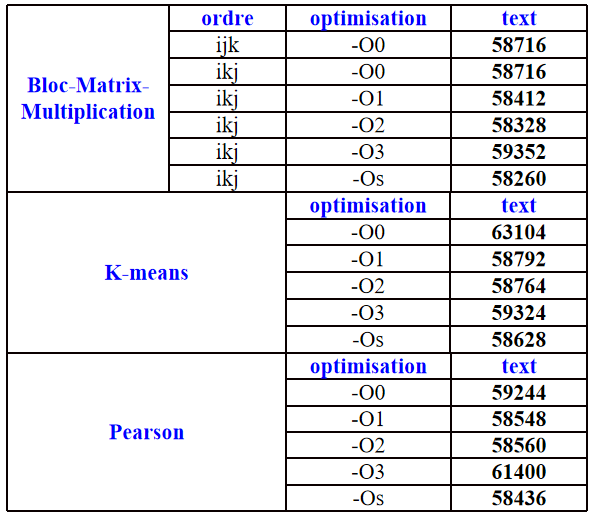
\includegraphics[width=0.6\linewidth]{soft/screenshot006}
	\caption{Un exemple des tailles de codes produit par l'optimisation}
	\label{fig:screenshot006}
\end{figure}
\begin{figure}[H]
	\centering
	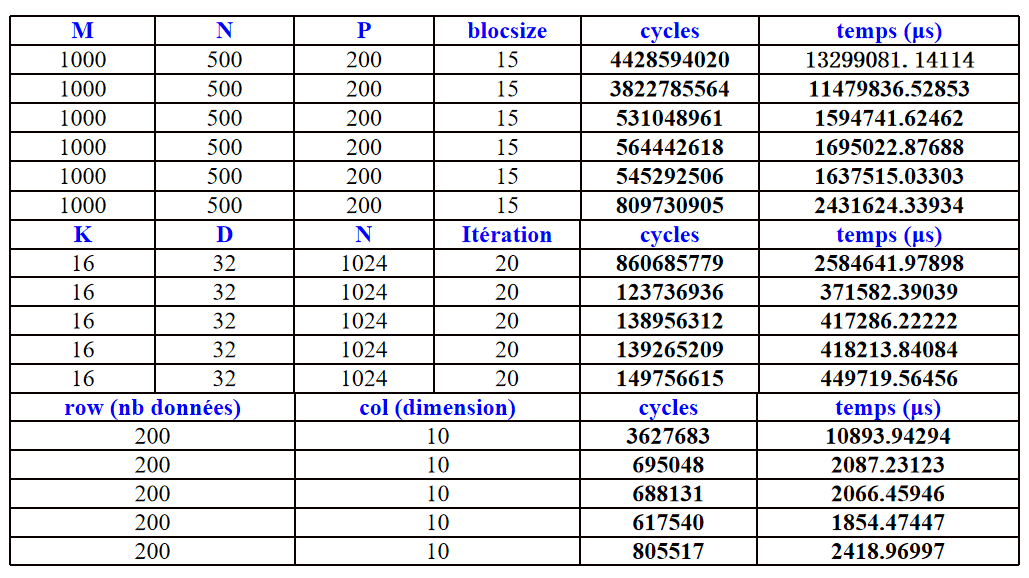
\includegraphics[width=\linewidth]{soft/screenshot007}
	\caption{Un exemple des temps d'exécution des codes produit par l'optimisation}
	\label{fig:screenshot007}
\end{figure}


\subsection{Performances HLS}
En mesurant le temps grâce au timer du \textit{Zynq}, on peut évaluer les performance des IPs.\\
Les IPs évaluées sont:
\begin{itemize}
	\item[•]Block matrix multiplication 32 par 32(\textit{mul32}) et 64 par 64(\textit{mul64})
	\item[•]Le coefficient de Pearson (\textit{pearson})
	\item[•]L'algorithme kmeans (\textit{kmeans})
\end{itemize}
\bigskip
On compare ainsi les temps Software, Hardware et Hardware avec clock amélioré:\\
\bigskip
\begin{tabular}{|c|c|c|c|c|}
	\hline
	\scriptsize exemple d'IP & \scriptsize temps HW ($\mu s$) @100MHZ & \scriptsize temps SW ($\mu s$) & \scriptsize fréquence améliorée & \scriptsize temps HW amélioré($\mu s$) \\ \hline
	mul64           &              10280.17417               &          26132.32432           &            130 MHZ             &          7042.11712 useconds           \\
	mul32           &               2411.54655               &           3281.83483           &             125MHZ             &               1809.89489               \\
	pearson          &                32.56906                &            5.25826             &            115 MHZ             &                21.19820                \\
	kmeans          &               1297.41742               &         1527.90390          &             120MHZ             &               1082.07808               \\ \hline
\end{tabular}\\
\bigskip
On a aussi essayé de serrer encore plus les timings en jouant sur la Clock des AXI et sur l'algorithme de placement (Haute performance). Avec les réglages suivants : 
\begin{itemize}
	\item[•]AXI\_CLK=180MHZ
	\item[•]HLS\_CLK=131MHZ
\end{itemize}
On a un temps de 6215.74174 $\mu s$ soit plus de 4 fois moins de temps que la version SW classique.



\subsection{Performances PC}
Pour comparaison, la figure \ref{fig:timepc} donne les performances en temps d'exécution pour différents paramètres des algorithmes.
\begin{figure}[H]
	\centering
	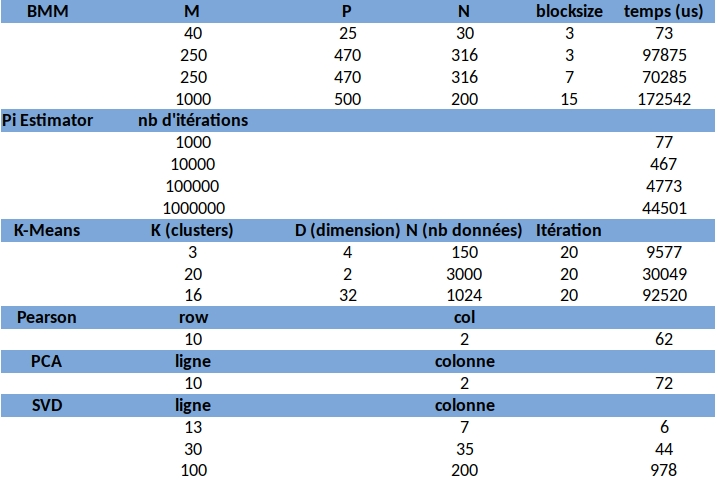
\includegraphics[width=0.8\linewidth]{soft/time_pc}
	\caption{Temps d'exécution sur PC}
	\label{fig:timepc}
\end{figure}
Il est évident que ces performances seront meilleures car les PC modernes sont multicœurs et sont cadencées à 3 GHz au minimum avec des optimisations de toutes sortes (exécution dans le désordre, prédiction des branchements, pipelines profonds, cache multi-niveaux...).

\section{Conclusion et perspectives}
Ce projet aura permis de découvrir une architecture hétérogène CPU+FPGA ainsi que les outils de développement qui lui dédié. On a pu implémenté les algorithmes de la série SPARK. L'exploration des possibilité et le choix des algorithmes étaient une étape assez délicate qui demandait l'accord de tous les membres de l'équipe. Ces implémentation en C on étaient exécutées sur PC et ARM avec des plus tentatives d'implémentation sur $\mu$blaze mais rendu impossible dans les délais déterminés à cause de problèmes au niveau des programmes de développement.

Certaines IPs HLS conçues montrent une inconsistance/incohérence lors de leurs exécutions ainsi que des différences de résultats, comme pour Kmeans, à cause des différentes normes utilisées et des arrondis. L'interfaçage de ces IPs est correctement assuré par la partie matérielle. On a pu montrer qu'une simple implémentation non optimisée d'une IP HLS est au minimum 4 fois plus rapide, sur la série d'algorithmes que l'on a fait, que l'exécution sur CPU. Il est aussi possible de cadencer les différentes IP du systèmes avec différentes horloges. Cette possibilité rend le système plus hétérogène qu'avant, le complexifiant certes, mais améliorant les performances en termes de temps. Il est aussi à constater que l'usage des IPs consomme plus de ressources s'elles ne sont pas agrégées. i.e. Il est souvent plus performant d'avoir une seule IP qui gèrent toutes l'implémentation RTL si les communications ne sont pas très fréquentes. Dans le cas contraire ceci saturerait l'interface de communication AXI. Enfin, la limite matérielle sur le FPGA reste le plafond physique pour ce genre de solution.


De manière similaire au projet, l'équipe est hétérogène et demandait un certain niveau de coopération. Plusieurs difficultés, concernant les logiciels de développement et un manque de performances des PCs utilisés, ont entravé le bon déroulement du projet. Il faut aussi noté que, malgré tous les efforts mis dans la coopération et communication mais aussi la séparation des tâches, on a rencontré quelques conflits de point de vu. Ceci est dû aux différentes habitudes de chaque membre de l'équipe.


En perspectives, on prévoit :

\begin{itemize}
\item \textbf{Implémentation sur $\mu$blaze} : On souhaite terminer l'implémentation logicielle des algorithmes sur un $\mu$blaze afin de comparer les performances à celles du ARM et de l'IP HLS. Ensuite, on envisage passer à une version multi-$\mu$-blazes où chacun des CPU exécute soit une partie du calcul ou un autre algorithme.
\item \textbf{HLS multi-IPs} : même si théoriquement une implémentation multi-IPs de sous-opérateurs semble moins bonne qu'une implémentation d'une IP unique, on souhaite effectuer plusieurs tests sur ces modèles afin d'avoir une base de comparaison.
\item \textbf{$\mu$blaze - HLS} On pense aussi avoir une implémentation multi-$\mu$blaze où chacun serait capable de contrôler une ou plusieurs IP HLS. Ceci répartirait la charge du calcul sur les $\mu$blazes et leur IPs mais risque de mener à un encombrement en communication.
\end{itemize}


\vfill
\textbf{code :} \href{https://github.com/anisghaoui/A2}{https://github.com/anisghaoui/A2}
\end{document}